\subsection{Decision Tree  and Extra-Tree Feature Generation}

In working with the decision trees, we utilized dimensionality reduction techniques including linear discriminant analysis (LDA) and principle components analysis (PCA) for training and testing classical decision trees, which pass over all features to consider which decision nodes to generate. This improved the computational requirements of the algorithm, as features in lower dimensions require less processing to distinguish.

LDA reduces data with $K$ classes in large dimensions (on the order of the number of pixels) to 
$K$ dimensions which captures the most energy of the data. Implementing LDA as dimensionality reduction, MNIST and Extended YaleB datasets are reduced to 10 and 38 variables respectively (for each data point.) We then worked with this transformed data as the input to our decision tree classifier for training and testing.

In a separate experiment, we considered the effects of utilizing the raw pixel data as features in \emph{extra-trees} which are ensembles of decision trees trained on randomly chosen features and thresholds. When testing, the mode of the predicted classes is chosen as the global prediction of the ensemble of trees. This method is shown to be more accurate than our classical decision trees trained on PCA- and LDA-generated features in Section (\ref{sec:results}).

\subsection{LDA vs PCA}

LDA and PCA linearly transform the data to reduce its dimensionality. Dimensionality reduction is helpful in many algorithms because it eases computational requirements and improves the generalizability of the classifier. This latter benefit is conferred by the manner in which dimensionality reduction smoothes out the individual variations in a particular class. A good dimensionality reduction algorithm should maximize the 'distance' between classes in the transformed (reduced) space, while minimizing the variance, or spread of those classes in the transformed space. 

The difference between the two techniques is that LDA is supervised whereas PCA is unsupervised. PCA finds orthogonal projections which capture the most variance of each feature, thereby expressing the data along \emph{principle components} that are the most distinct. We can visually exemplify the PCA technique as in the figure below. 

	\begin{figure}[H]
		\centering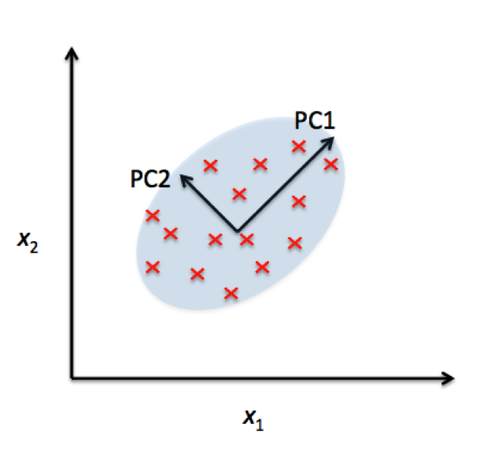
\includegraphics[width=0.4\textwidth]{../images/pca}
		\caption{PCA implemented on 2-dimensional data \cite{images:ldapca}. }
	\end{figure}

        In our PCA implementation, we rely on the \emph{singular value decomposition} (SVD) to generate our features, conventionally described as \emph{scores}. To perform the singular value decomposition and obtain our features, we must first pre-process the data. We arrange it so that the rows of our data $X$ are the individual images in the dataset, with each column corresponding to a pixel value. Then, we subtract the column-wise empirical mean from each column to render each column zero-mean. Then, we utilize MATLAB's built-in \code{svd(.)} to obtain the matrices $[U, S, V]$. Our features are represented by $U*S$. Taking the transpose of this matrix, and extracting the first $n$ columns, where $n$ is the number of features we seek to utilize, we have a matrix of features corresponding to each image in our dataset. This method was useful, although not as effective in training decision trees as LDA, which we now discuss.

LDA maximizes the class separability and can be represented visually as in the figure below. 
	\begin{figure}[H]
	\centering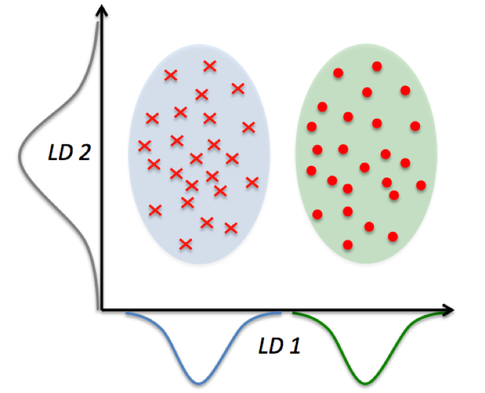
\includegraphics[width=0.4\textwidth]{../images/lda}
	\caption{LDA visualization \cite{images:ldapca}.}
	\end{figure}
        The underlying concept of LDA is taking the eigenvectors of $ \dfrac{\Sigma_b}{\Sigma_w}$ where $\Sigma_w$ is within-class scatter matrix and $\Sigma_b$ is between-class scatter matrix. This division of matrices separates the classes away from one another. This is distinct from PCA, which is unsupervised, thereby only capturing the data in a minimum number of variables irrespective of class. Please see Section (\ref{sec:lda}) for more information on LDA.
